% ======================================================================
% capitulos/linea2/e4_calidad.tex
% ----------------------------------------------------------------------
% LÍNEA CE02 — INGENIERÍA DE SOFTWARE
% S2 · E4: GESTIÓN DEL PROYECTO Y CALIDAD DE SOFTWARE (alineado con CE024)
% Fuentes: anexos/WISP-reporte-de-pruebas.pdf (rama pastor, commit dd46fc1, 19/11/2026);
%          ejecución reproducida: datos/pruebas/pytest_2026-11-19.txt y junit_2026-11-19.xml;
%          métricas: radon 6.0.1 y ruff 0.6.9 sobre backend/app; historial git del repositorio;
%          pipeline propuesto: config/ci_wisp.yml
% ======================================================================
\chapter{Gestión del Proyecto y Calidad de Software}
\label{chap:ce02-e4}

\entregable{CE02 --- Ingeniería de Software · competencia CE024 Calidad de Software}
{Semestre 2 · Entregable 4: Gestión del Proyecto y Calidad de Software}
{CE0241 Suite de pruebas automatizadas · CE0242 Pipeline de integración, despliegue y operación continua · CE0243 Gestión ágil del proyecto de software · CE0244 Aseguramiento y auditoría de la calidad}
{Pruebas ejecutadas y reproducidas (121 unitarias, 45 de API, 308 de interfaz). Pipeline CI diseñado y validado contra el código, por activar en el repositorio.}

\begin{table}[H]
\centering
\caption{Datos de la versión evaluada.}
\label{tab:ce02-e4-ficha}
\small
\begin{tabularx}{\textwidth}{L{3.6cm}X}
\toprule
Sistema & WISP Control --- panel web, API REST y base de datos \\
Versión probada & Rama \texttt{pastor}, commit \texttt{dd46fc1} (19/11/2026) \\
Entorno de pruebas & Docker local \texttt{wisp-local}: FastAPI + PostgreSQL 15 + panel React 19 \\
Herramientas & pytest 9.2 + pytest-cov 7.1 (líneas y ramas), Chrome sin interfaz por DevTools Protocol, radon 6.0.1, ruff 0.6.9 \\
Reporte fuente & \texttt{WISP-reporte-de-pruebas.pdf}, 25 páginas (anexo al final del capítulo) \\
\bottomrule
\end{tabularx}
\end{table}

\section*{Resumen ejecutivo}
\addcontentsline{toc}{section}{Resumen ejecutivo}

\textbf{Calidad del producto.} El sistema se probó en tres niveles: 121 pruebas unitarias y
de caja blanca, 45 casos de caja negra contra la API y 308 verificaciones de caja negra en la
interfaz, con 732 decisiones de permiso revisadas una a una. \textbf{Todo pasa.} La ronda
encontró y corrigió dos defectos reales: el ``corte temporal'' de pagos se rechazaba siempre y
un estado de ONU no cumplía el contraste mínimo WCAG AA. Las reglas críticas del negocio
(facturación, cobro mensual y permisos) tienen 100\,\% de cobertura de líneas y ramas. La
cobertura total del backend es de 41\,\%, porque los módulos que hablan con MikroTik y WhatsApp
se prueban de punta a punta en la interfaz con respuestas simuladas.

\textbf{Operación.} El sistema funciona en producción (\texttt{wispfibra.com}) con
contenedores que se reinician solos, verificación de salud de la base y de la API, límites de
recursos y respaldo diario de la base. La integración todavía es manual: se trabaja en ramas y
se despliega con \texttt{git pull} y Docker Compose. Se diseñó un pipeline de integración
continua de cuatro etapas, validado contra el código actual. Su primer resultado esperado es
señalar 26 hallazgos de análisis estático que deben corregirse antes de activarlo.

\textbf{Proceso.} El proyecto se gestiona con un enfoque híbrido PMBOK + Scrum, cuyo Project
Charter, EDT, cronograma y riesgos están en el \cref{chap:plangestion}. Este capítulo agrega la
evidencia del semestre~2: el backlog actualizado con el estado real de cada historia, los dos
sprints de construcción reconstruidos desde los 95 commits que contienen, su retrospectiva y la
comparación con RUP, Cascada y Kanban.

\textbf{Aseguramiento.} Se aplicó una matriz de calidad basada en ISO/IEC 25010 con métricas
medidas, se midió el código con radon y ruff, se registró la deuda técnica y se auditó el
proceso con una lista de verificación de áreas de proceso de CMMI-DEV (método tipo SCAMPI~C,
autoevaluación). El proceso cumple casi todo el nivel~2 de madurez, pero le faltan
aseguramiento formal y medición sistemática. El plan de mejora cierra esas brechas.

\begin{table}[H]
\centering
\caption{Estado frente a la rúbrica del entregable.}
\label{tab:ce02-e4-rubrica}
\small
\begin{tabularx}{\textwidth}{L{4.2cm}L{2.2cm}X}
\toprule
\textbf{Criterio} & \textbf{Estado} & \textbf{Evidencia} \\
\midrule
Cobertura y calidad de pruebas & Completo & 474 casos en tres niveles; reglas críticas al 100\,\%; ejecución reproducida (\cref{sec:ce02-e4-pruebas}). \\
Automatización (CI/CD) & Parcial & Pruebas automatizadas y despliegue con un comando; pipeline CI diseñado y validado, por activar (\cref{sec:ce02-e4-cicd}). \\
Operación y observabilidad & Funcional & Salud, reinicio automático, registros, límites, respaldo diario y rollback documentado; faltan alertas automáticas. \\
Gestión ágil & Completo & Charter (CE01), backlog con estado real, sprint backlog, métricas y retrospectiva (\cref{sec:ce02-e4-agil}). \\
Comparación de marcos & Completo & Scrum frente a RUP, Cascada y Kanban, con la adaptación usada (\cref{tab:ce02-e4-marcos}). \\
Aseguramiento de la calidad & Completo & Matriz ISO/IEC 25010, instrumentos y métricas de código (\cref{sec:ce02-e4-calidad}). \\
Auditoría de madurez (CMMI) & Completo & Lista de verificación por área de proceso, deuda técnica y plan de mejora. \\
Sustentación & Pendiente & Exposición ante el docente. \\
\bottomrule
\end{tabularx}
\end{table}

% ======================================================================
\section{Sección 1: Pruebas}
\label{sec:ce02-e4-pruebas}

\subsection{Estrategia}

Se probó en tres niveles complementarios. Las \textbf{pruebas unitarias} revisan funciones y
endpoints aislados con una base SQLite en memoria que se crea y se borra en cada prueba, sin
tocar datos reales. Las de \textbf{caja blanca} miran el código por dentro: miden qué líneas y
ramas se ejecutaron y recorren a propósito cada camino de las reglas críticas. Las de
\textbf{caja negra} ignoran el código y solo comparan entradas con salidas, en la API y en la
interfaz, con clases de equivalencia, valores límite y tablas de decisión.

\begin{table}[H]
\centering
\caption{Niveles de prueba, técnicas y resultados.}
\label{tab:ce02-e4-niveles}
\small
\begin{tabularx}{\textwidth}{L{2.6cm}XC{1.6cm}C{1.8cm}}
\toprule
\textbf{Nivel} & \textbf{Qué se probó y cómo} & \textbf{Casos} & \textbf{Resultado} \\
\midrule
Unitarias & Inventario, ONUs, pagos, gastos, ciclo de servicio del cliente y reglas puras. pytest + FastAPI TestClient. & 121 & 121 pasan \\
Caja blanca & Cobertura de líneas y ramas (\texttt{--cov-branch}); caminos de permisos, facturación y validación; matriz de permisos; migraciones de ida y vuelta. & 732 decisiones & Sin regresiones \\
Caja negra · API & Autenticación, permisos por rol, validación de ONU, inventario y pagos. Peticiones HTTP reales al servidor en Docker. & 45 & 45 pasan \\
Caja negra · interfaz & 9 recorridos completos en Chrome a 1440~px, a 390~px (teléfono) y en modo oscuro, sin errores de JavaScript. & 308 & 308 pasan \\
\bottomrule
\end{tabularx}
\end{table}

Las pruebas no afectan la operación: los envíos de WhatsApp y las consultas a los MikroTik se
interceptan y se responden con datos simulados, y lo que las pruebas crean se borra al
terminar.

\subsection{Reporte de ejecución}

Para este documento se volvió a ejecutar la suite en el mismo entorno, el 19/11/2026, con el
comando que deja el reporte. Los resultados coinciden con el reporte del equipo. La salida
completa está en \texttt{datos/pruebas/pytest\_2026-11-19.txt} y el resultado de cada caso,
en formato JUnit, en \texttt{junit\_2026-11-19.xml}.

\begin{lstlisting}[style=plano]
$ docker exec wisp_local_backend sh -c "cd /app && python -m pytest -q tests/ \
      --cov=app --cov-branch --junitxml=/tmp/junit.xml"
...
app/acceso.py                      69      0     14      0   100%
app/billing.py                     19      0      6      0   100%
app/facturacion.py                 18      0      2      0   100%
app/onus_historial.py              36      2     16      1    94%
TOTAL                            6707   3562   1712    113    41%
121 passed, 129 warnings in 7.45s
\end{lstlisting}

\begin{table}[H]
\centering
\caption{Pruebas unitarias por archivo.}
\label{tab:ce02-e4-unitarias}
\small
\begin{tabularx}{\textwidth}{L{4.6cm}XC{1.2cm}}
\toprule
\textbf{Archivo} & \textbf{Qué cubre} & \textbf{Casos} \\
\midrule
\texttt{test\_clientes\_servicio.py} & Ciclo de servicio: cortar, reactivar, pausar, aprobar e instalar (router y WhatsApp simulados). & 19 \\
\texttt{test\_gastos.py} & Gastos: alta, recurrentes, filtros, edición y borrado. & 18 \\
\texttt{test\_inventario.py} & Entregas, devoluciones, consumo, todo-o-nada, piezas con etiqueta, lector, unidades. & 20 \\
\texttt{test\_onus.py} & Validación de serie y MAC, repetidas, historial, traspaso, borrado protegido. & 23 \\
\texttt{test\_pagos.py} & Corte temporal, pago normal, adelantos, duplicados. & 12 \\
\texttt{test\_reglas\_unitarias.py} & Reglas puras: facturación, cobro mensual y decisión de permisos. & 29 \\
\midrule
\textbf{Total} & & \textbf{121} \\
\bottomrule
\end{tabularx}
\end{table}

\subsection{Cobertura de código}

\begin{table}[H]
\centering
\caption{Cobertura de líneas y ramas por módulo (pytest-cov, \texttt{--cov-branch}).}
\label{tab:ce02-e4-cobertura}
\small
\begin{tabularx}{\textwidth}{XC{2cm}C{2cm}C{2cm}}
\toprule
\textbf{Módulo} & \textbf{Líneas} & \textbf{Ramas} & \textbf{Cobertura} \\
\midrule
\texttt{facturacion.py} · día de pago y vencimientos & 18/18 & 2/2 & 100,0\,\% \\
\texttt{billing.py} · monto mensual y desglose & 19/19 & 6/6 & 100,0\,\% \\
\texttt{acceso.py} · decisión de permisos & 69/69 & 14/14 & 100,0\,\% \\
\texttt{onus\_historial.py} · validación de serie y MAC & 34/36 & 15/16 & 94,2\,\% \\
\texttt{routers/inventario.py} & 333/386 & 122/158 & 83,6\,\% \\
\texttt{routers/onus.py} & 145/181 & 42/66 & 75,7\,\% \\
\texttt{routers/gastos.py} & 65/87 & 17/24 & 73,9\,\% \\
\texttt{routers/pagos.py} & 186/417 & 32/118 & 40,7\,\% \\
\texttt{routers/clientes.py} & 260/873 & 61/364 & 25,9\,\% \\
\midrule
\textbf{Paquete \texttt{app} completo} & 3145/6707 & 345/1712 & \textbf{41,5\,\%} \\
\bottomrule
\end{tabularx}
\end{table}

La cobertura se concentra donde un error cuesta dinero o expone datos: el cálculo de lo que
paga cada cliente, su fecha de pago y quién puede hacer qué. Los routers con menor cobertura
(zonas, WhatsApp, MikroTik, jornadas y parte de clientes) dependen de servicios externos y hoy
se prueban de punta a punta en la interfaz. Subir esa cobertura es la primera meta del plan
de mejora (\cref{tab:ce02-e4-mejora}).

\subsection{Caja blanca: caminos y matriz de permisos}

Los casos se diseñaron leyendo el código para pasar por cada rama de las reglas críticas.

\begin{table}[H]
\centering
\caption{Caminos recorridos a propósito en las reglas críticas.}
\label{tab:ce02-e4-caminos}
\small
\begin{tabularx}{\textwidth}{L{4.2cm}X}
\toprule
\textbf{Función} & \textbf{Ramas recorridas} \\
\midrule
\texttt{acceso.permite\_con\_roles} & Ruta sin regla; superadministrador; regla ``amplia'' (basta el módulo); regla ``usar'' (módulo y tipo de cuenta, falta uno u otro); los módulos de Red no abren escrituras. \\
\texttt{acceso.modulo\_disponible} & Cliente, admin, solo-admin, técnico, vendedora, delegable y atención (10 casos). \\
\texttt{facturacion.dia\_de\_pago} & Día $\le$ 25 y día $\ge$ 26 (pasa al 1): límites 1, 25, 26 y 31. \\
\texttt{facturacion.con\_dia} & Mes corto, febrero bisiesto y no bisiesto. \\
\texttt{facturacion.primer\_vencimiento} & Rama normal (+1 mes) y rama del 26 (+2 meses al día 1). \\
\texttt{billing.monto\_mensual} & Sin plan, sin TV adicional, con TV adicional y TV nula. \\
\texttt{onus\_historial.normalizar\_*} & Serie corta, hexadecimal de la OLT, larga e inválida; MAC con separadores, vacía, ceros, multicast y no hexadecimal. \\
\bottomrule
\end{tabularx}
\end{table}

\paragraph{Matriz de permisos.} Un script recorre todas las rutas de la API y, para cada tipo
de cuenta (administrador, técnico, vendedora de campo y atención al cliente), compara la
decisión real del sistema con la esperada según los módulos de su rol: \textbf{732
decisiones}. Las únicas 30 diferencias son endpoints nuevos de Inventario, ONUs y Cajas NAP que
quedan cerrados para quien no tiene el módulo, que es lo esperado. Ninguna decisión que ya
existía cambió.

\paragraph{Migraciones.} Cada migración nueva de Alembic se aplicó, se revirtió y se volvió a
aplicar sobre PostgreSQL con datos, sin errores. Entre ellas está la que reconstruye el
historial de las 58 ONUs existentes. Esta prueba es la base del rollback de la base de datos
(\cref{sec:ce02-e4-rollback}).

\subsection{Caja negra: API e interfaz}

\begin{table}[H]
\centering
\caption{Casos representativos de caja negra sobre la API (45 de 45 pasan).}
\label{tab:ce02-e4-api}
\small
\begin{tabularx}{\textwidth}{L{2cm}L{2.4cm}XC{1.5cm}C{1.5cm}}
\toprule
\textbf{Grupo} & \textbf{Técnica} & \textbf{Caso y entrada} & \textbf{Esperado} & \textbf{Obtenido} \\
\midrule
Autenticación & Equivalencia (inválida) & Contraseña incorrecta & 401 & 401 \\
Autenticación & Valor límite & Usuario y contraseña vacíos & 401/422 & 422 \\
Autenticación & Equivalencia (inválida) & Token alterado & 401 & 401 \\
Permisos & Tabla de decisión & Técnico sin módulo consulta el stock & 403 & 403 \\
Permisos & Tabla de decisión & Técnico consulta su propio material & 200 & 200 \\
ONU · serie & Valor límite & 11 y 13 caracteres (uno menos, uno más) & rechazada & rechazada \\
ONU · MAC & Equivalencia & Todo ceros, difusión y multicast & rechazada & rechazada \\
Inventario & Valor límite & Entregar el stock + 1 & 400 & 400 \\
Inventario & Valor límite & Cantidad 0 y cantidad $-5$ & 422 & 422 \\
Pagos & Valor límite & Monto $-1$ y monto 0 & 400 & 400 \\
Pagos & Equivalencia (inválida) & Cliente inexistente & 404 & 404 \\
\bottomrule
\end{tabularx}
\end{table}

\begin{table}[H]
\centering
\caption{Recorridos de caja negra en la interfaz (308 de 308 pasan).}
\label{tab:ce02-e4-ui}
\small
\begin{tabularx}{\textwidth}{L{3.2cm}XC{1.2cm}}
\toprule
\textbf{Recorrido} & \textbf{Qué cubre} & \textbf{Casos} \\
\midrule
Inventario & Stock, movimientos, piezas con etiqueta, lector, unidades, cifras & 60 \\
ONUs & Alta con validación, tanda, ficha, entrega, traspaso, daño, recuperación & 41 \\
Caja NAP & Puertos, inspector, dañado/reparado, precinto, router & 24 \\
Zonas y cajas & Filtros, orden, vista de lista, detalle desde la lista & 28 \\
Red / Inventario & Red solo consulta; Inventario gestiona & 19 \\
Módulos padre & Crear, mover, menú agrupado y por rol & 35 \\
WhatsApp masivo & Envío en tres pasos (interceptado) & 22 \\
ONU y consumo & Corregir la MAC y registrar consumo con cliente & 11 \\
Diseño y accesibilidad & Contraste claro/oscuro, desborde, foco, en todas las pantallas & 68 \\
\bottomrule
\end{tabularx}
\end{table}

\begin{figure}[H]
\centering
\fbox{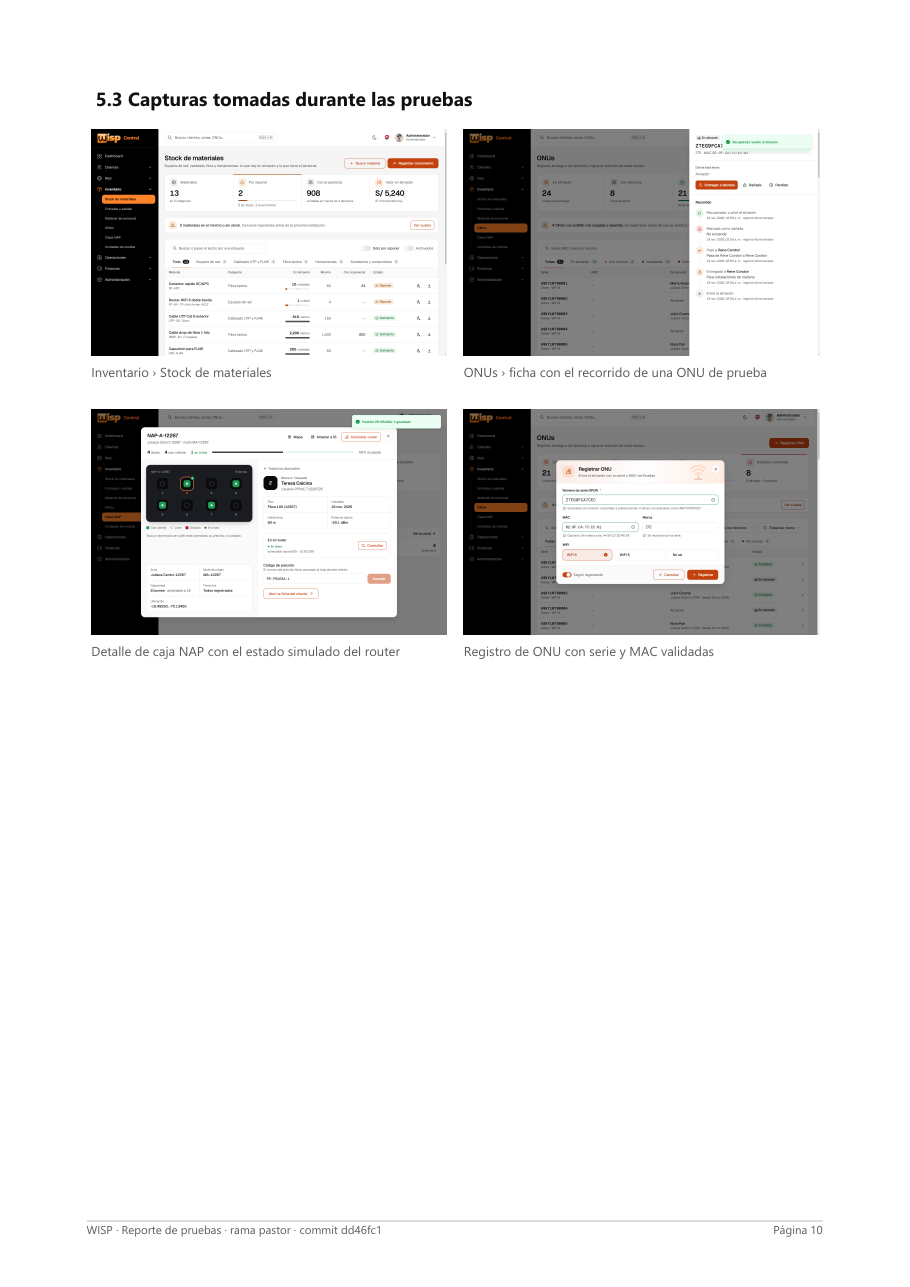
\includegraphics[width=0.78\textwidth]{linea2/calidad/rep-10.png}}
\caption{Capturas tomadas por las pruebas de interfaz durante los recorridos (página 10 del reporte).}
\label{fig:ce02-e4-capturas}
\end{figure}

\subsection{Pruebas sobre flujos críticos y defectos}

\begin{table}[H]
\centering
\caption{Trazabilidad entre flujos críticos del negocio y pruebas.}
\label{tab:ce02-e4-flujos}
\small
\begin{tabularx}{\textwidth}{L{3.6cm}L{2.6cm}X}
\toprule
\textbf{Flujo crítico} & \textbf{Requisitos} & \textbf{Pruebas que lo cubren} \\
\midrule
Aprobar e instalar un cliente & RF-10, RF-11, RN-05 & \texttt{test\_aprobar\_un\_pendiente}, \texttt{test\_no\_se\_aprueba\_dos\_veces}, \texttt{test\_instalar\_exige\_que\_este\_aprobado} \\
Corte y reactivación & RF-33 a RF-35, RN-07 a RN-09 & \texttt{test\_cortar\_suspende\_avisa\_y\_luego\_corta\_en\_el\_router}, \texttt{test\_reactivar\_no\_perdona\_la\_deuda}, corte con IP fija \\
Cobro y fecha de pago & RF-29, RF-32, RN-06 & 29 reglas puras al 100\,\%; pagos duplicados, adelantos, montos límite \\
Control de acceso & RN-04, RN-12 & 732 decisiones de la matriz; 8 casos de permisos en la API \\
Inventario de ONUs y materiales & RF-24 a RF-26, RN-02 & \texttt{test\_entrega\_de\_varias\_lineas\_es\_todo\_o\_nada}, validación de serie y MAC, devoluciones y consumo con tope \\
\bottomrule
\end{tabularx}
\end{table}

\begin{table}[H]
\centering
\caption{Defectos encontrados en la ronda de pruebas.}
\label{tab:ce02-e4-defectos}
\small
\begin{tabularx}{\textwidth}{C{0.6cm}XL{3.4cm}L{1.6cm}}
\toprule
\textbf{\#} & \textbf{Defecto} & \textbf{Detectado por} & \textbf{Estado} \\
\midrule
1 & Pagos: el ``corte temporal'' (un mes sin servicio, monto 0) se rechazaba siempre, porque una regla posterior exigía monto mayor que cero para todo registro. & Unitarias: 3 pruebas de \texttt{TestCorteTemporal} fallaban con 400 & Corregido \\
2 & ONUs: el estado ``Con técnico'' tenía contraste 4,48:1, debajo del mínimo WCAG AA de 4,5:1. & Interfaz: verificación de contraste & Corregido \\
\bottomrule
\end{tabularx}
\end{table}

\noindent Además, cuatro verificaciones de interfaz se ajustaron porque el sistema cambió
legítimamente; en esos casos se corrigió la prueba, no la aplicación. Por ejemplo, se agregaron
dos módulos (de 23 a 25) y una caja ya estaba en su capacidad máxima.

\paragraph{Limitaciones.} No se probó contra MikroTik ni WhatsApp reales; sus respuestas se
simularon para no afectar a los clientes. La app Expo no entra en esta ronda. Tampoco se
hicieron pruebas de carga más allá del bloqueo de filas en movimientos de stock. El tiempo de
respuesta en producción se midió aparte (\cref{sec:ce02-e3-desempeno}).

% ======================================================================
\section{Sección 2: Integración, despliegue y operación continua}
\label{sec:ce02-e4-cicd}

\subsection{Cómo se integra y despliega hoy}

\begin{table}[H]
\centering
\caption{Práctica actual de integración y despliegue.}
\label{tab:ce02-e4-actual}
\small
\begin{tabularx}{\textwidth}{L{3.2cm}X}
\toprule
\textbf{Práctica} & \textbf{Cómo se hace} \\
\midrule
Control de versiones & Git en GitHub (\texttt{cristian-csc/Wisp-ISP}). \texttt{main} es lo que está en producción; \texttt{pastor} es la rama de trabajo. 97 commits del 19/10 al 19/11/2026. \\
Integración & Cada cambio se prueba en el Docker local (\texttt{docker-compose.local.yml}, igual al de producción) antes de unirlo a \texttt{main}. \\
Pruebas & Suite automatizada en \texttt{backend/tests/} (121 casos en 7,5~s); scripts de caja negra de API e interfaz. Se ejecutan a mano antes de integrar. \\
Despliegue & Un comando: \texttt{git pull} y \texttt{docker compose \ldots{} up -d --build}. Las migraciones de Alembic se aplican solas al arrancar el backend. Existe además \texttt{scripts/deploy.sh}. \\
Publicación & Cloudflare Tunnel: el servidor no abre puertos de entrada, así que un despliegue no cambia la exposición. \\
App móvil & Compilación con EAS (\texttt{eas build}). \\
\bottomrule
\end{tabularx}
\end{table}

La integración continua \textbf{todavía no es automática}: nada impide unir a \texttt{main} un
cambio cuyas pruebas fallan. Para cerrar esa brecha se diseñó el pipeline siguiente.

\subsection{Pipeline CI/CD propuesto}

El pipeline está escrito para GitHub Actions (\texttt{config/ci\_wisp.yml}, destino
\texttt{.github/workflows/ci.yml}) y se ejecuta en cada \emph{push} y \emph{pull request}. Cada
paso se comprobó contra el repositorio actual. Existen \texttt{backend/requirements.txt},
\texttt{frontend/package-lock.json} y el script \texttt{build} (\texttt{tsc -b \&\& vite
build}); las pruebas pasan, y la cobertura de las tres reglas críticas es 100\,\%, así que el
umbral se cumple.

\begin{figure}[H]
\centering
\begin{tikzpicture}[font=\scriptsize]
\node[caja, text width=2.1cm] (push) at (0,0) {\textbf{Push / PR}\\ a \texttt{main} o \texttt{pastor}};
\node[caja, text width=3.6cm] (be) at (4.0,2.0) {\textbf{Backend}\\ ruff · pytest + cobertura\\ umbral 100\,\% en reglas críticas};
\node[caja, text width=3.6cm] (mig) at (4.0,0) {\textbf{Migraciones}\\ PostgreSQL 15\\ upgrade · downgrade · upgrade};
\node[caja, text width=3.6cm] (fe) at (4.0,-2.0) {\textbf{Frontend}\\ \texttt{npm ci} · tipos\\ build de producción};
\node[caja, text width=2.1cm] (img) at (7.9,0) {\textbf{Imágenes}\\ \texttt{docker compose build}};
\node[cajasec, text width=2.9cm] (cd) at (11.3,0) {\textbf{Despliegue (CD)}\\ el servidor tira de \texttt{main}, verifica salud y revierte si falla};
\draw[flecha] (push) -- (be.west); \draw[flecha] (push) -- (mig); \draw[flecha] (push) -- (fe.west);
\draw[flecha] (be.east) -- (img); \draw[flecha] (mig) -- (img); \draw[flecha] (fe.east) -- (img);
\draw[flecha] (img) -- (cd);
\end{tikzpicture}
\caption{Etapas del pipeline propuesto.}
\label{fig:ce02-e4-pipeline}
\end{figure}

\begin{lstlisting}[style=plano]
backend:      ruff check app --select F,B904,E711,E712 --ignore B008
              python -m pytest -q tests/ --cov=app --cov-branch --junitxml=junit.xml
              coverage report --include="app/acceso.py,app/billing.py,app/facturacion.py" \
                              --fail-under=100
migraciones:  alembic upgrade head && alembic downgrade -1 && alembic upgrade head
frontend:     npm ci && npm run build
imagenes:     docker compose -f docker-compose.yml build backend frontend web whatsapp
\end{lstlisting}

\paragraph{Por qué el despliegue es ``de tirar'' y no ``de empujar''.} El servidor está en la
oficina detrás de Cloudflare Tunnel y no acepta conexiones de entrada, que es una decisión de
seguridad del SGSI. Por eso GitHub no puede entrar a desplegar. Se propone que el propio
servidor revise cada 15 minutos si \texttt{main} avanzó con el CI en verde y, en ese caso,
cree una etiqueta de la versión anterior, actualice, reconstruya y verifique
\texttt{/api/health}. Si la verificación falla, vuelve solo a la etiqueta anterior.

\paragraph{Primer resultado esperado.} Con las reglas de análisis estático elegidas, el
pipeline hoy fallaría por 26 hallazgos reales: 10 \texttt{raise} sin \texttt{from}, 8
comparaciones con \texttt{True}/\texttt{False}, 6 imports sin usar y 2 comparaciones con
\texttt{None}. Dieciséis se corrigen automáticamente con \texttt{ruff --fix}. Es la primera
tarea del plan de mejora y la condición para activar el pipeline.

\subsection{Evidencias de integración}

\begin{figure}[H]
\centering
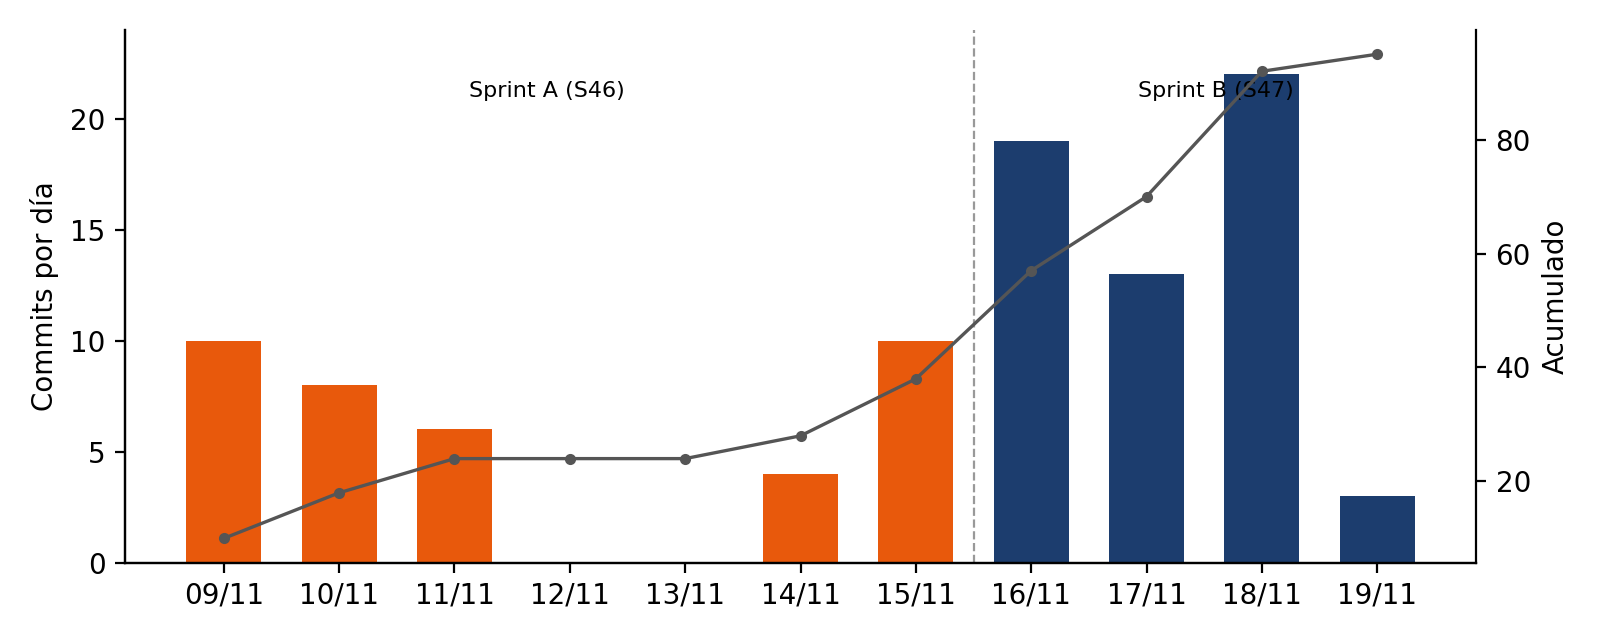
\includegraphics[width=0.92\textwidth]{linea2/calidad/commits_dia.png}
\caption{Commits integrados por día durante los dos sprints de construcción (historial git).}
\label{fig:ce02-e4-commits}
\end{figure}

El historial muestra integración frecuente y en lotes pequeños: 95 commits en 11 días, con
mensajes que describen el cambio (``Corrige migración que falla en una base nueva'',
``Advierte sobre la regla de cortafuegos que deja la API en 504''). Participan dos autores
principales (73 y 20 commits) y 4 commits sin autor configurado, que también se registran
como hallazgo.

\subsection{Observabilidad en producción}

\begin{table}[H]
\centering
\caption{Observabilidad: lo que existe y lo que falta.}
\label{tab:ce02-e4-observabilidad}
\small
\begin{tabularx}{\textwidth}{L{2.6cm}XL{1.8cm}}
\toprule
\textbf{Señal} & \textbf{Implementación} & \textbf{Estado} \\
\midrule
Salud & \texttt{healthcheck} de PostgreSQL (\texttt{pg\_isready}); endpoint \texttt{GET /api/health}; el backend espera a que la base esté sana. & Operativo \\
Autorrecuperación & \texttt{restart: unless-stopped} en los 7 contenedores; el panel resuelve la API por DNS de Docker y la encuentra aunque se reinicie. & Operativo \\
Registros (logs) & 14 \emph{loggers} en el backend; \texttt{docker compose logs} por servicio; registro de \texttt{cloudflared} con el estado del túnel. & Operativo \\
Métricas de recursos & \texttt{docker stats}; techo de 0,5 CPU y 512~MB para WhatsApp. & Operativo \\
Métricas de negocio & Dashboard del panel: clientes activos, cobrado del mes, por instalar, averías, pagos pendientes (\cref{fig:ce02-e3-dashboard}). & Operativo \\
Estado de la red & Estado del túnel WireGuard de cada zona y diagnóstico de planes contra los routers, desde el panel. & Operativo \\
Tiempo de respuesta & Medición reproducible con \texttt{tools/medir\_desempeno.py} (\cref{sec:ce02-e3-desempeno}). & Manual \\
Alertas & No hay aviso automático si el sitio cae. Propuesta: monitor externo (Uptime Kuma o Healthchecks.io) cada minuto sobre \texttt{/api/health} con aviso por WhatsApp/correo al administrador. & Falta \\
\bottomrule
\end{tabularx}
\end{table}

\subsection{Estrategia de rollback y respaldos}
\label{sec:ce02-e4-rollback}

\begin{table}[H]
\centering
\caption{Cómo se vuelve atrás según lo que falló.}
\label{tab:ce02-e4-rollback}
\small
\begin{tabularx}{\textwidth}{L{3cm}X}
\toprule
\textbf{Qué falló} & \textbf{Cómo se revierte} \\
\midrule
Una versión del código & \texttt{git checkout <commit o etiqueta anterior>} y \texttt{docker compose up -d --build}. Las imágenes son reproducibles desde el repositorio. \\
Una migración & \texttt{alembic downgrade -1}. Cada migración nueva se probó de ida y vuelta (\cref{sec:ce02-e4-pruebas}). \\
Datos dañados o borrados & Restaurar el respaldo diario: \texttt{pg\_dump} comprimido a las 03:00, retención de 30 días y copia fuera del servidor (\cref{chap:ce02-datos}, ``Estrategias de respaldo y recuperación''). \\
El servidor completo & Reinstalar en otro equipo con el manual técnico (\cref{sec:ce02-e3-manual}) y restaurar base y evidencias; el túnel se reconecta con el mismo token. \\
Una zona (router) & La configuración de cada MikroTik se respalda aparte (plan de continuidad del SGSI, \cref{chap:ce03-sgsi}). \\
\bottomrule
\end{tabularx}
\end{table}

% ======================================================================
\section{Sección 3: Gestión ágil del proyecto de software}
\label{sec:ce02-e4-agil}

\subsection{Project Charter}

El Project Charter se elaboró en el semestre~1 y no se repite aquí. La
\cref{tab:ce02-e4-charter} indica dónde está cada elemento y qué cambió en el semestre~2.

\begin{table}[H]
\centering
\caption{Elementos del Project Charter y su actualización.}
\label{tab:ce02-e4-charter}
\small
\begin{tabularx}{\textwidth}{L{2.6cm}L{2.8cm}X}
\toprule
\textbf{Elemento} & \textbf{Dónde está} & \textbf{Actualización del semestre 2} \\
\midrule
Acta y objetivos & \cref{sec:acta}, \cref{tab:objetivos-acta} & Objetivos vigentes; el sistema ya opera en producción. \\
Alcance y EDT & \cref{tab:edt} & Se agregaron Inventario de materiales, historial de ONUs, roles configurables y WhatsApp masivo. Se postergó la validación de comprobantes con IA. \\
Equipo y roles & \cref{tab:roles-scrum} & Sin cambios: PO, Scrum Master y dos desarrolladores. \\
Cronograma & \cref{tab:gantt}, \cref{tab:sprints} & Los sprints de construcción se detallan abajo. \\
Riesgos & \cref{tab:riesgos-identificacion} & Riesgo nuevo de calidad: integración sin CI (tratado en el plan de mejora). \\
\bottomrule
\end{tabularx}
\end{table}

\subsection{Product Backlog actualizado}

El backlog del semestre~1 (\cref{tab:backlog}) se actualizó con el estado real de cada historia
según el código, y con las historias que surgieron durante la construcción.

\begin{table}[H]
\centering
\caption{Product Backlog con estado al 19/11/2026.}
\label{tab:ce02-e4-backlog}
\small
\begin{tabularx}{\textwidth}{L{1.1cm}XC{1.2cm}L{1.8cm}}
\toprule
\textbf{ID} & \textbf{Historia de usuario} & \textbf{Prior.} & \textbf{Estado} \\
\midrule
HU-01 & Como vendedor, registrar prospectos desde la app móvil. & Alta & Hecho \\
HU-02 & Como administrador, validar prospectos y aprobar la venta (crea el PPPoE). & Alta & Hecho \\
HU-03 & Como técnico, registrar la instalación (caja, borne, ONU, fotos) desde la app. & Alta & Hecho \\
HU-04 & Como administrador, cortar y reactivar clientes en el MikroTik desde el sistema. & Alta & Hecho \\
HU-05 & Como administrador, gestionar clientes, planes y zonas desde el panel. & Media & Hecho \\
HU-06 & Como visitante, ver planes y cobertura en el sitio web. & Media & Hecho \\
HU-07 & Como cliente, recibir recordatorios de pago por WhatsApp. & Baja & Hecho \\
HU-08 & Como administrador, definir roles y qué módulos ve cada uno. & Alta & Hecho \\
HU-09 & Como almacenero, controlar stock, entregas y consumo de materiales. & Alta & Hecho \\
HU-10 & Como administrador, seguir el recorrido de cada ONU. & Media & Hecho \\
HU-11 & Como administrador, enviar avisos masivos por WhatsApp. & Media & Hecho \\
HU-12 & Como técnico, ver mufas y cajas NAP en el mapa de la zona. & Media & Hecho \\
HU-13 & Como administrador, comparar los planes del panel con los perfiles de cada router. & Media & Hecho \\
HU-14 & Como técnico, reportar una ONU dañada y avisar al administrador (RF-27, RF-28). & Media & Parcial \\
HU-15 & Como cliente, consultar mis pagos y vencimientos (RF-44 a RF-46). & Media & Parcial \\
HU-16 & Como administrador, coordinar la fecha de instalación por WhatsApp (RF-08, RF-13, RF-14). & Baja & Pendiente \\
HU-17 & Como cliente, enviar mi comprobante y que se valide solo con IA (RF-39 a RF-43). & Baja & Pendiente \\
\bottomrule
\end{tabularx}
\end{table}

\subsection{Sprint Backlog y métricas de avance}

Los sprints de construcción del semestre~2 se reconstruyeron desde el historial del
repositorio. Cada commit se asignó a su semana ISO y a un tema según su mensaje.

\begin{table}[H]
\centering
\caption{Sprint Backlog de los sprints de construcción (commits por tema).}
\label{tab:ce02-e4-sprints}
\small
\begin{tabularx}{\textwidth}{XC{2.6cm}C{2.6cm}}
\toprule
\textbf{Tema (historias)} & \textbf{Sprint A}\newline 09--15/11 (S46) & \textbf{Sprint B}\newline 16--22/11 (S47) \\
\midrule
Zonas, red y planes (HU-05, HU-13) & 11 & 16 \\
Roles y módulos (HU-08) & 7 & 3 \\
Mapa e infraestructura (HU-12) & 5 & 7 \\
Despliegue y seguridad & 5 & 1 \\
Clientes y pagos (HU-02, HU-04) & 2 & 10 \\
Inventario y ONUs (HU-09, HU-10) & --- & 5 \\
WhatsApp (HU-07, HU-11) & 1 & 3 \\
Pruebas y accesibilidad & --- & 1 \\
Otros (ajustes de interfaz) & 7 & 11 \\
\midrule
\textbf{Total de commits} & \textbf{38} & \textbf{57} \\
\textbf{Incremento} & Roles configurables; despliegue en \texttt{wispfibra.com} & Inventario, ONUs, mapa, diagnóstico de planes; ronda de pruebas \\
\bottomrule
\end{tabularx}
\end{table}

\begin{table}[H]
\centering
\caption{Métricas de avance del proyecto de software.}
\label{tab:ce02-e4-metricas}
\small
\begin{tabularx}{\textwidth}{L{5.6cm}C{2.4cm}X}
\toprule
\textbf{Métrica} & \textbf{Valor} & \textbf{Lectura} \\
\midrule
Historias hechas / total & 13 / 17 (76\,\%) & Las 7 historias del semestre~1 están hechas. \\
Requisitos funcionales implementados & 41 / 56 (73\,\%) & Más 5 parciales (\cref{tab:ce02-rf}). \\
Commits por sprint (A $\rightarrow$ B) & 38 $\rightarrow$ 57 & El ritmo subió un 50\,\%. \\
Defectos encontrados / corregidos & 2 / 2 & Ninguno abierto. \\
Pruebas que pasan & 474 / 474 & Unitarias, API e interfaz. \\
\bottomrule
\end{tabularx}
\end{table}

\subsection{Ceremonias y retrospectiva}

Las ceremonias siguen lo definido en el semestre~1 (\cref{sec:scrum}): planificación al
inicio de cada sprint, coordinación diaria del equipo, revisión del incremento con el Product
Owner y retrospectiva. La revisión del Sprint~B se apoya en evidencia verificable: el reporte
de pruebas y el sistema en producción. La retrospectiva siguiente se elaboró a partir de esa
evidencia, y el equipo debe validarla y firmarla en su acta.

\begin{table}[H]
\centering
\caption{Retrospectiva del Sprint B.}
\label{tab:ce02-e4-retro}
\small
\begin{tabularx}{\textwidth}{L{3cm}X}
\toprule
\textbf{Pregunta} & \textbf{Respuesta del equipo} \\
\midrule
¿Qué salió bien? & El sistema llegó a producción sin abrir puertos. La ronda de pruebas encontró 2 defectos antes de que los viera un usuario. Las migraciones se probaron de ida y vuelta. \\
¿Qué no salió bien? & Las pruebas se ejecutan a mano: un cambio puede llegar a \texttt{main} sin pasar por ellas. Cuatro verificaciones quedaron desactualizadas por cambios de la interfaz. Hay 4 commits sin autor configurado. \\
¿Qué haremos distinto? & Activar el CI y exigirlo antes de unir a \texttt{main}; mover los scripts de caja negra al repositorio; configurar \texttt{git config user.name} en todos los equipos. \\
\bottomrule
\end{tabularx}
\end{table}

\subsection{Comparación y adaptación de marcos de proceso}

\begin{table}[H]
\centering
\caption{Comparación de marcos de proceso aplicada al proyecto.}
\label{tab:ce02-e4-marcos}
\small
\begin{tabularx}{\textwidth}{L{2.5cm}*{4}{>{\raggedright\arraybackslash}X}}
\toprule
\textbf{Aspecto} & \textbf{Scrum (adoptado)} & \textbf{RUP} & \textbf{Cascada} & \textbf{Kanban} \\
\midrule
Ciclo de vida & Iterativo en sprints cortos & Iterativo en 4 fases (Inicio, Elaboración, Construcción, Transición) & Secuencial, una sola entrega & Flujo continuo, sin iteraciones \\
Requisitos & Backlog que cambia & Casos de uso estables en Elaboración & Fijos al inicio & Tarjetas según llegan \\
Roles & PO, SM, desarrolladores & Muchos roles por disciplina & Por fase & No prescribe \\
Documentación & Mínima & Abundante (artefactos por disciplina) & Abundante por fase & Mínima \\
Ajuste a WISP & Alto: el negocio cambia y el equipo es pequeño & Medio: buena arquitectura, pero pesado para 4 personas & Bajo: el alcance cambió en S2 & Alto para operación y soporte \\
\bottomrule
\end{tabularx}
\end{table}

\paragraph{Adaptación usada.} El proyecto combina tres marcos según la etapa:
\begin{itemize}
  \item \textbf{PMBOK} para la gestión formal del semestre~1: acta, EDT, costos y riesgos
  (\cref{chap:plangestion}).
  \item \textbf{Scrum} para construir el software en sprints con incrementos desplegables.
  \item \textbf{Kanban} para la operación: averías, instalaciones y pagos pendientes se
  gestionan como flujo continuo con la bandeja ``Por atender'' del panel.
\end{itemize}
De \textbf{RUP} se tomaron dos prácticas de su fase de Elaboración: fijar pronto la
arquitectura, con el modelo C4 y 9 ADR (\cref{chap:ce02-e1}), y modelar los datos antes de
construir (\cref{chap:ce02-datos}). Las semanas del semestre~1 corresponden a las fases de
Inicio y Elaboración; las del semestre~2, a Construcción y Transición.

% ======================================================================
\section{Sección 4: Aseguramiento y auditoría de la calidad del software}
\label{sec:ce02-e4-calidad}

\subsection{Matriz de calidad (ISO/IEC 25010)}

\begin{table}[H]
\centering
\caption{Matriz de calidad: atributo, métrica, meta, valor medido y riesgo.}
\label{tab:ce02-e4-matriz}
\small
\begin{tabularx}{\textwidth}{L{2.4cm}L{3.2cm}C{1.5cm}C{1.7cm}X}
\toprule
\textbf{Atributo} & \textbf{Métrica} & \textbf{Meta} & \textbf{Medido} & \textbf{Riesgo si falla} \\
\midrule
Adecuación funcional & RF implementados & $\ge$ 80\,\% & 73\,\% (+9\,\% parcial) & Procesos que siguen en papel o WhatsApp \\
Corrección funcional & Pruebas que pasan & 100\,\% & 100\,\% (474) & Cobros o cortes erróneos \\
Eficiencia & Procesamiento de la API & $<$ 50 ms & 3--7 ms & Panel lento en horas de cobro \\
Eficiencia & Tiempo con conexión abierta & $<$ 500 ms & $\approx$ 229 ms & Mala experiencia en campo \\
Fiabilidad & Peticiones con éxito & 100\,\% & 150/150 & Pérdida de ventas o pagos \\
Seguridad & Decisiones de permiso correctas & 100\,\% & 732/732 & Acceso indebido a datos personales \\
Seguridad & Cobertura de \texttt{acceso.py} & 100\,\% & 100\,\% & Escalada de privilegios \\
Mantenibilidad & Complejidad ciclomática media & A ($\le$ 5) & A (3,64) & Cambios costosos \\
Mantenibilidad & Funciones con complejidad $>$ 10 & 0 & 34 de 587 & Errores al modificar \\
Capacidad de prueba & Cobertura total de ramas & $\ge$ 60\,\% & 20\,\% & Regresiones sin detectar \\
Usabilidad & Contraste WCAG AA & 100\,\% & 100\,\% (tras corrección) & Pantallas ilegibles al sol \\
Portabilidad & Instalación con un comando & Sí & Sí (Docker Compose) & Dependencia de un equipo \\
\bottomrule
\end{tabularx}
\end{table}

\subsection{Instrumentos de aseguramiento}

\begin{table}[H]
\centering
\caption{Instrumentos de aseguramiento de la calidad.}
\label{tab:ce02-e4-instrumentos}
\small
\begin{tabularx}{\textwidth}{L{3.4cm}X}
\toprule
\textbf{Instrumento} & \textbf{Cómo se aplica} \\
\midrule
Definición de Terminado & Criterio de aceptación cumplido, probado, versionado y revisado por el PO (\cref{sec:scrum}). \\
Revisión de código & Antes de unir \texttt{pastor} a \texttt{main}, otro integrante revisa el cambio con la lista de la \cref{tab:ce02-e4-checklist-codigo}. \\
Inspección de interfaz & Recorridos de caja negra con verificación de contraste, desborde y foco en todas las pantallas. \\
Análisis estático & radon (complejidad, mantenibilidad) y ruff (\emph{code smells}); en el CI, ruff bloquea. \\
Matriz de permisos & Comparación automática de 732 decisiones ante cada cambio de roles o rutas. \\
Medición de desempeño & \texttt{tools/medir\_desempeno.py} después de cada despliegue. \\
\bottomrule
\end{tabularx}
\end{table}

\begin{table}[H]
\centering
\caption{Lista de verificación para la revisión de código.}
\label{tab:ce02-e4-checklist-codigo}
\small
\begin{tabularx}{\textwidth}{C{0.7cm}X}
\toprule
\textbf{\#} & \textbf{Verificación} \\
\midrule
1 & El cambio corresponde a una historia del backlog y cumple su criterio de aceptación. \\
2 & La suite pasa completa y el cambio trae pruebas de sus ramas nuevas. \\
3 & Toda ruta nueva tiene regla de acceso en \texttt{acceso.py} y aparece en la matriz de permisos. \\
4 & Las migraciones nuevas se aplican y se revierten sin error. \\
5 & No hay contraseñas, llaves ni datos personales en el código ni en los commits. \\
6 & Las entradas se validan con Pydantic; los errores devuelven 4xx con mensaje claro. \\
7 & Ninguna función nueva supera complejidad 10 sin justificación. \\
8 & La pantalla funciona a 390~px y en modo oscuro, con contraste AA. \\
\bottomrule
\end{tabularx}
\end{table}

\subsection{Calidad del código, \emph{code smells} y deuda técnica}

Se midió el backend (\texttt{backend/app}, rama \texttt{pastor}) con radon y ruff.

\begin{table}[H]
\centering
\caption{Métricas internas del código del backend.}
\label{tab:ce02-e4-codigo}
\small
\begin{tabularx}{\textwidth}{L{5.2cm}C{2.2cm}X}
\toprule
\textbf{Métrica} & \textbf{Valor} & \textbf{Lectura} \\
\midrule
Líneas de código fuente (SLOC) & 9\,910 & 13\,170 líneas físicas. \\
Comentarios y docstrings & 10\,\% & Aceptable; las reglas críticas están documentadas. \\
Bloques analizados & 587 & Funciones, métodos y clases. \\
Complejidad ciclomática media & 3,64 (A) & La mayoría del código es simple. \\
Bloques por rango A / B / C / D / E & 491 / 62 / 23 / 8 / 3 & 34 bloques en C o peor. \\
Índice de mantenibilidad más bajo & \texttt{clientes.py} (C) & 1\,968 líneas en un solo router. \\
Componentes del panel más grandes & 1\,842 / 1\,471 / 955 líneas & \texttt{ClienteDetail}, \texttt{ZonaDetail}, \texttt{Pagos}. \\
\bottomrule
\end{tabularx}
\end{table}

\begin{table}[H]
\centering
\caption{\emph{Code smells} detectados y su tratamiento.}
\label{tab:ce02-e4-smells}
\small
\begin{tabularx}{\textwidth}{L{3.2cm}C{1.2cm}X}
\toprule
\textbf{Smell} & \textbf{Casos} & \textbf{Tratamiento} \\
\midrule
Método largo y complejo & 16 & \texttt{registrar\_movimientos} (CC 40), \texttt{create\_pago} (36), \texttt{instalar\_cliente} (33): extraer validaciones y efectos a funciones de servicio. \\
Clase o módulo dios & 3 & \texttt{clientes.py}, \texttt{pagos.py}, \texttt{inventario.py}: dividir por caso de uso (alta, servicio, instalación). \\
Excepción sin causa & 10 & \texttt{raise HTTPException(...) from e} para no perder la traza. \\
Comparación con \texttt{True}/\texttt{None} & 10 & Usar \texttt{.is\_(True)} y \texttt{is None}; corrección automática. \\
Import sin usar & 6 & Eliminar; corrección automática. \\
API heredada & 9 & \texttt{Query.get()} genera 129 avisos de SQLAlchemy 2.0: cambiar a \texttt{Session.get()}. \\
Llamada en argumento por defecto & 497 & \emph{Falso positivo}: es el patrón \texttt{Depends()} de FastAPI; se excluye (B008). \\
\bottomrule
\end{tabularx}
\end{table}

\begin{table}[H]
\centering
\caption{Registro de deuda técnica.}
\label{tab:ce02-e4-deuda}
\small
\begin{tabularx}{\textwidth}{L{1cm}XC{1.4cm}L{3.4cm}}
\toprule
\textbf{ID} & \textbf{Deuda} & \textbf{Impacto} & \textbf{Refactorización} \\
\midrule
DT-01 & Cobertura baja en routers que llaman a MikroTik y WhatsApp & Alto & Simular los clientes SSH y HTTP en pruebas unitarias \\
DT-02 & Routers de clientes y pagos demasiado grandes & Medio & Capa de servicios por caso de uso \\
DT-03 & 26 hallazgos de análisis estático & Bajo & \texttt{ruff --fix} y corrección manual \\
DT-04 & Uso de \texttt{Query.get()} heredado & Bajo & Migrar a \texttt{Session.get()} \\
DT-05 & Estado en memoria (freno de login, caché WG, planificador) & Medio & Redis y planificador único (\cref{sec:ce02-e3-escalabilidad}) \\
DT-06 & Scripts de caja negra fuera del repositorio & Medio & Moverlos a \texttt{tests/e2e/} \\
DT-07 & Imagen \texttt{cloudflared:latest} sin versión fija & Medio & Fijar versión (NC-07 del SGSI) \\
\bottomrule
\end{tabularx}
\end{table}

\noindent La deuda ya se gestiona con refactorización. En esta ronda, el defecto~1 se corrigió
reordenando las validaciones de \texttt{create\_pago}. La historia del inventario pasó de
cantidades sueltas a piezas con etiqueta sin perder lo que cada técnico tenía a su cargo, y una
prueba lo garantiza (\texttt{test\_etiquetar\_material\_existente\_respeta\_lo\_que\_tiene\_cada\_uno}).

\subsection{Auditoría técnica y madurez del proceso (CMMI-DEV)}

\paragraph{Método.} Autoevaluación al estilo SCAMPI clase~C: revisión documental y de
artefactos (repositorio, reporte de pruebas, este documento), sin entrevistas formales ni
equipo evaluador externo. Para cada área de proceso de los niveles 2 y 3 de CMMI-DEV v1.3 se
calificó la evidencia como \textbf{S} (satisfecha), \textbf{P} (parcial) o \textbf{N} (no
satisfecha).

\begin{table}[H]
\centering
\caption{Lista de verificación de auditoría por área de proceso CMMI-DEV.}
\label{tab:ce02-e4-cmmi}
\small
\begin{tabularx}{\textwidth}{L{1.1cm}L{3.2cm}XC{0.6cm}}
\toprule
\textbf{Área} & \textbf{Pregunta de auditoría} & \textbf{Evidencia encontrada} & \textbf{Cal.} \\
\midrule
\multicolumn{4}{l}{\cellcolor{upeublue!10}\textbf{Gestión de proyecto (nivel 2)}} \\
PP & ¿Hay plan con alcance, estimación y riesgos? & Charter, EDT, cronograma, costos y riesgos (\cref{chap:plangestion}) & S \\
PMC & ¿Se compara el avance con el plan? & Backlog con estado, métricas por sprint; sin informe periódico formal & P \\
REQM & ¿Se gestionan y trazan los requisitos? & 56 RF con estado según el código; trazabilidad a pruebas (\cref{tab:ce02-e4-flujos}) & S \\
\multicolumn{4}{l}{\cellcolor{upeublue!10}\textbf{Soporte (nivel 2)}} \\
CM & ¿Hay control de versiones y de líneas base? & Git, ramas \texttt{main}/\texttt{pastor}, migraciones versionadas; sin etiquetas de versión & P \\
PPQA & ¿Alguien verifica objetivamente el proceso? & Lista de revisión definida; sin registro de revisiones hechas & P \\
MA & ¿Se miden y analizan indicadores? & Cobertura, complejidad, desempeño y commits medidos en esta auditoría; no de forma periódica & P \\
\multicolumn{4}{l}{\cellcolor{upeublue!10}\textbf{Ingeniería (nivel 3)}} \\
RD & ¿Los requisitos se desarrollan y validan? & SRS, RNF y reglas de negocio (\cref{chap:ce02-e1}) & S \\
TS & ¿Las decisiones técnicas están justificadas? & C4 y 9 ADR & S \\
PI & ¿La integración es planificada y repetible? & Docker Compose reproducible; integración no automatizada & P \\
VER & ¿Se verifica el producto? & 474 casos, revisión de permisos, análisis estático & S \\
VAL & ¿Se valida con el usuario? & Sistema en producción usado por WISP; acta de validación por firmar & P \\
\bottomrule
\end{tabularx}
\end{table}

\paragraph{Resultado.} El proceso está en \textbf{nivel~1 con la mayor parte del nivel~2
alcanzado}: PP y REQM están satisfechas, pero PMC, CM, PPQA y MA son parciales, y el nivel~2
exige las seis. En ingeniería (nivel~3) destacan RD, TS y VER. La brecha no está en la
calidad técnica, sino en hacer el proceso \emph{repetible y registrado}: automatizar la
integración, etiquetar versiones y llevar registro de revisiones y métricas.

\begin{table}[H]
\centering
\caption{Hallazgos de la auditoría técnica.}
\label{tab:ce02-e4-hallazgos}
\small
\begin{tabularx}{\textwidth}{L{1.3cm}L{1.6cm}X}
\toprule
\textbf{ID} & \textbf{Tipo} & \textbf{Hallazgo} \\
\midrule
AQ-01 & No conformidad & No hay CI: un cambio puede llegar a producción sin pasar las pruebas (PI, PPQA). \\
AQ-02 & No conformidad & No hay etiquetas de versión ni notas de cambios: no se sabe qué versión está en producción sin consultar el servidor (CM). \\
AQ-03 & Observación & 4 commits sin autor identificado (CM). \\
AQ-04 & Observación & Las métricas se miden en auditorías, no en cada sprint (MA). \\
AQ-05 & Observación & Las revisiones de código no dejan registro (PPQA). \\
AQ-06 & Fortaleza & Reglas críticas al 100\,\% de cobertura y matriz completa de permisos. \\
AQ-07 & Fortaleza & Pruebas que no tocan servicios reales y migraciones probadas de ida y vuelta. \\
\bottomrule
\end{tabularx}
\end{table}

\subsection{Plan de mejora de la calidad del software}

\begin{table}[H]
\centering
\caption{Plan de mejora de la calidad.}
\label{tab:ce02-e4-mejora}
\small
\begin{tabularx}{\textwidth}{C{0.6cm}XL{2cm}L{2cm}L{2.4cm}}
\toprule
\textbf{\#} & \textbf{Acción} & \textbf{Atiende} & \textbf{Plazo} & \textbf{Indicador} \\
\midrule
1 & Corregir los 26 hallazgos de ruff y activar el pipeline CI como requisito para unir a \texttt{main} & AQ-01, DT-03 & Semana 1 & CI en verde \\
2 & Etiquetar cada despliegue (\texttt{v1.0.0}\ldots) con notas de cambios & AQ-02 & Semana 1 & 1 etiqueta por despliegue \\
3 & Monitor externo con alerta por WhatsApp sobre \texttt{/api/health} & Observabilidad & Semana 2 & Aviso en $<$ 2 min \\
4 & Pruebas unitarias de zonas, MikroTik y WhatsApp con clientes simulados & DT-01 & Semanas 2--4 & Cobertura $\ge$ 60\,\% \\
5 & Mover scripts de caja negra a \texttt{tests/e2e/} y ejecutarlos en CI & DT-06 & Semana 3 & 353 casos en CI \\
6 & Dividir \texttt{clientes.py} y \texttt{pagos.py} en servicios & DT-02 & Semanas 3--6 & Ninguna función con CC $>$ 20 \\
7 & Revisiones de código en \emph{pull requests} con la lista de verificación & AQ-05 & Continuo & 100\,\% de PR revisados \\
8 & Tablero de métricas por sprint (cobertura, complejidad, defectos) & AQ-04 & Cada sprint & Informe en la revisión \\
9 & Pruebas de la app Expo (componentes y recorridos) & Limitación & Semestre siguiente & Suite móvil creada \\
\bottomrule
\end{tabularx}
\end{table}

% ======================================================================
\section*{Anexos del entregable}
\addcontentsline{toc}{section}{Anexos del entregable}
\label{sec:ce02-e4-anexos}

\begin{table}[H]
\centering
\caption{Anexos y dónde se encuentran.}
\label{tab:ce02-e4-anexos}
\small
\begin{tabularx}{\textwidth}{L{4.6cm}X}
\toprule
\textbf{Anexo} & \textbf{Ubicación} \\
\midrule
Reporte de pruebas & Páginas principales a continuación; completo en \texttt{anexos/WISP-reporte-de-pruebas.pdf} (25 págs., con la lista de cada caso) \\
Ejecución reproducida & \texttt{datos/pruebas/pytest\_2026-11-19.txt}, \texttt{junit\_2026-11-19.xml} \\
Pipeline CI & \texttt{config/ci\_wisp.yml} \\
Artefactos ágiles & Charter y backlog del semestre~1 (\cref{chap:plangestion}); \cref{tab:ce02-e4-backlog,tab:ce02-e4-sprints,tab:ce02-e4-retro} \\
Matriz de calidad y checklists & \cref{tab:ce02-e4-matriz,tab:ce02-e4-checklist-codigo,tab:ce02-e4-cmmi} \\
Evidencia de sustentación & Pendiente: exposición ante el docente \\
\bottomrule
\end{tabularx}
\end{table}

\subsection*{Reporte de pruebas (páginas 1 a 11)}
\label{sec:ce02-e4-anexo-reporte}

\includepdf[pages=1-11, scale=0.82, frame, pagecommand={\thispagestyle{fancy}}]{anexos/WISP-reporte-de-pruebas.pdf}
